\documentclass[a4paper, oneside, final]{scrartcl}

\usepackage{scrlayer-scrpage}
\usepackage{titlesec}
\usepackage{anysize}
\usepackage{marvosym}
\usepackage{tabularx,colortbl}
\usepackage{ebgaramond}
\usepackage{microtype}
\usepackage{hyperref}
\usepackage{graphicx}
\usepackage{amsmath}

\titleformat{\section}{\large\scshape\raggedright}{}{0em}{}[\titlerule]

\pagestyle{scrheadings}

\addtolength{\voffset}{-0.5in}
\addtolength{\textheight}{3cm}

\newcommand{\gray}{\rowcolor[gray]{.90}}

\renewcommand{\headfont}{\normalfont\rmfamily}

\marginsize{2cm}{2cm}{2cm}{2cm}
\setlength{\parindent}{0cm}

\begin{document}

\thispagestyle{empty}

\begin{center}
    %\newcommand{\HRule}{\rule{\linewidth}{0.5mm}}
    \begin{minipage}{0.29\textwidth} 
        \center{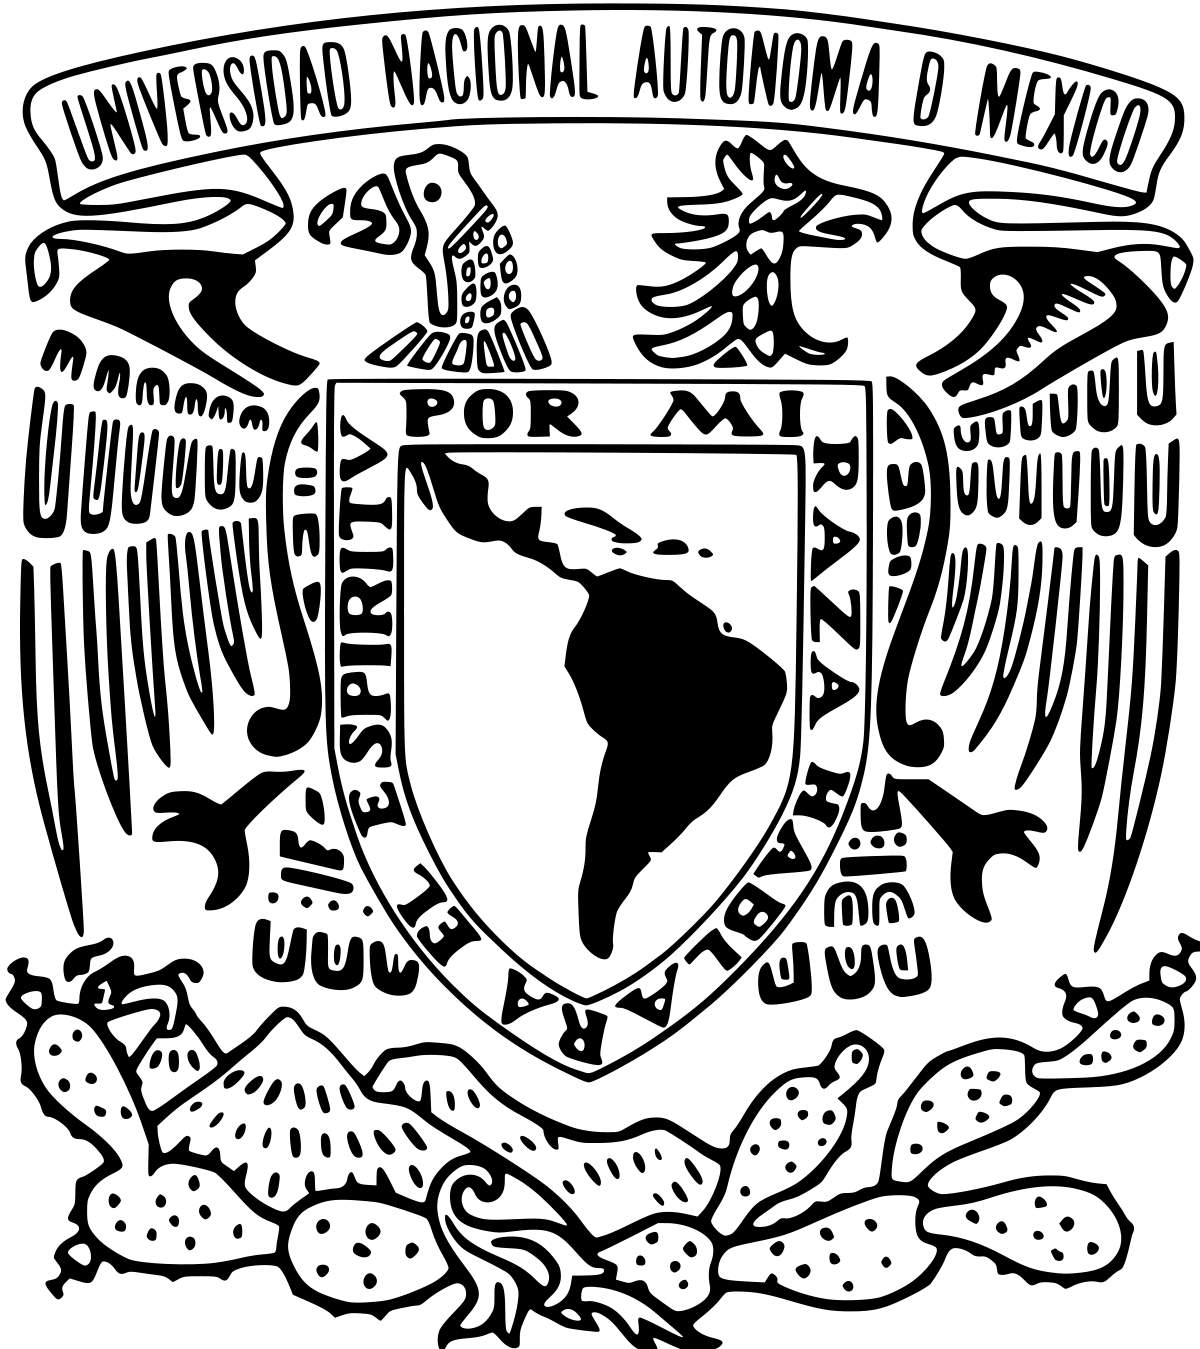
\includegraphics[scale = 0.06]{images/logo_unam.png}}
    \end{minipage}
    \begin{minipage}{0.40\textwidth} 
    \center{\textsc{\LARGE Universidad Nacional \\[5mm] Autónoma de México}}\\
    \end{minipage}
    \begin{minipage}{0.29\textwidth}
        \center{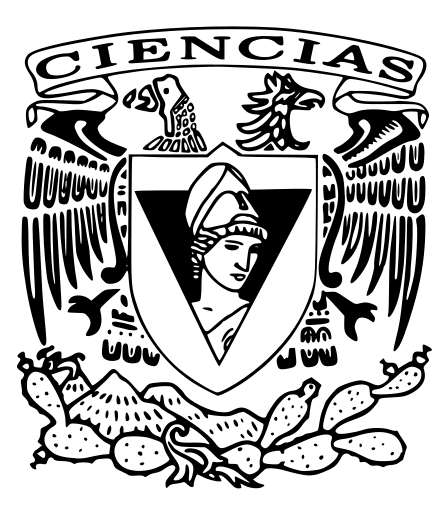
\includegraphics[scale =0.18]{images/logo_ciencias.png}}
    \end{minipage}
    \vspace{5mm}					
    
    \textsc{\noindent \LARGE Facultad de Ciencias}\\[20mm]
    
    \textsc{\LARGE   Ingeniería de Software \\[5mm]
                    \LARGE 2024-2}      \\[20mm]
    
    \textsc{\textbf{\huge   Análisis de requerimientos}}\\[5mm]
    \textsc{\LARGE  Pizarra colaborativa para computólogos}\\[20mm]

    \LARGE
    \textsc{Equipo I}\\[5mm]
    \Large 
    \textsc{Diego Sebastián Sánchez Correa}\\[2mm]
    \textsc{Mauro Emiliano Chávez Zamora}\\[2mm]
    \textsc{Ulises Josué Anaya Pérez}\\[2mm]
    \textsc{Daniel Linares Gil} \\[2mm]
    \textsc{Karyme Ivette Azpeitia García}
    \\[20mm]

    \large Creado: 15/02/2024\\[2mm]
    \large Última actualización: 20/02/2024\\
    
\end{center}	
\newpage  


\section{Resumen}

Se pretende proporcionar una herramienta básica que busca satisfacer las
necesidades esenciales para el desarrollo de proyectos relacionados con las ciencias de la computación.\\

La idea de un editor de texto con \textit{syntax highlighting} es común dentro
del ámbito de desarrollo de software, sin embargo, se carece de herramientas de
planeación colaborativa donde las ideas se puedan aterrizar de manera general o
con detalles tan específicos como los usuarios lo deseen.\\

Esta aplicación tiene como fin la creación de un ambiente colaborativo y cuya
esencia sirva como punto de partida para la elaboración de decisiones de diseño
a partir de diagramas, control de versiones, edición con dibujo vectorizado y
soporte para \LaTeX.
Ejemplos de herramientas de pizarra colaborativa: \href{https://miro.com/}{Miro}, \href{https://www.mural.co/}{Mural}, \href{ https://www.microsoft.com/en-us/microsoft-365/microsoft-whiteboard/digital-whiteboard-app}{Microsoft Whiteboard},\href{https://www.figma.com/figjam/}{Figjam} y \href{https://jamboard.google.com}{Jamboard}.

\section{Ejemplos de uso:}

\textbf{Entrevista de programación:} Alice se encuentra entrevistando candidatos para unirse a su equipo como
    desarrolladores de software. Alice decide utilizar nuestra pizarra colaborativa porque permite bloques de código,
    dibujar de manera libre y escribir diagramas para explicar la solución. Durante la entrevista, el candidato escribe
    su solución en el bloque de código y además puede utilizar las funcionalidades de diagramado y dibujo libre para explicar su solución a Alice.

\textbf{Reunión de retrospectiva:} Alice se prepara para la reunión de retrospectiva de su equipo de desarrollo luego de un sprint. Alice crea una nueva pizarra, y la divide en tres columnas:

\begin{itemize}
    \item ¿Qué fue bien?
    \item ¿Qué no fue bien?
    \item ¿Qué se puede mejorar?
\end{itemize}

Cuando Alice haya terminado de preparar la pizarra para la reunión, crea un enlace para compartir la pizarra y lo comparte con los miembros de su equipo. Durante la reunión, los miembros del equipos colaboran añadiendo notas en cada columna. También pueden incluir enlaces a los tickets de Jira correspondientes en las notas. Una vez terminan de añadir notas, los miembros del equipo discuten sobre estas.
\clearpage
\section{Requerimientos}

\textbf{\large Integración de Diagramas y Codificación}\\ %diego

  Provee un ambiente donde los desarrolladores pueden crear diagramas y escribir
  código en el mismo lugar, facilitando con ello la visualización y la
  implementación simultánea de ideas.

  Desde conceptos matemáticos simples como la incorporación de autómatas, hasta
  la integración de diagramas de flujo permitirán que los usuarios puedan ser
  capaces de definir las bases, algoritmos y diseño de un proyecto cuya esencia
  tenga una naturaleza colaborativa.

    \begin{figure}[h!]
    \centering
    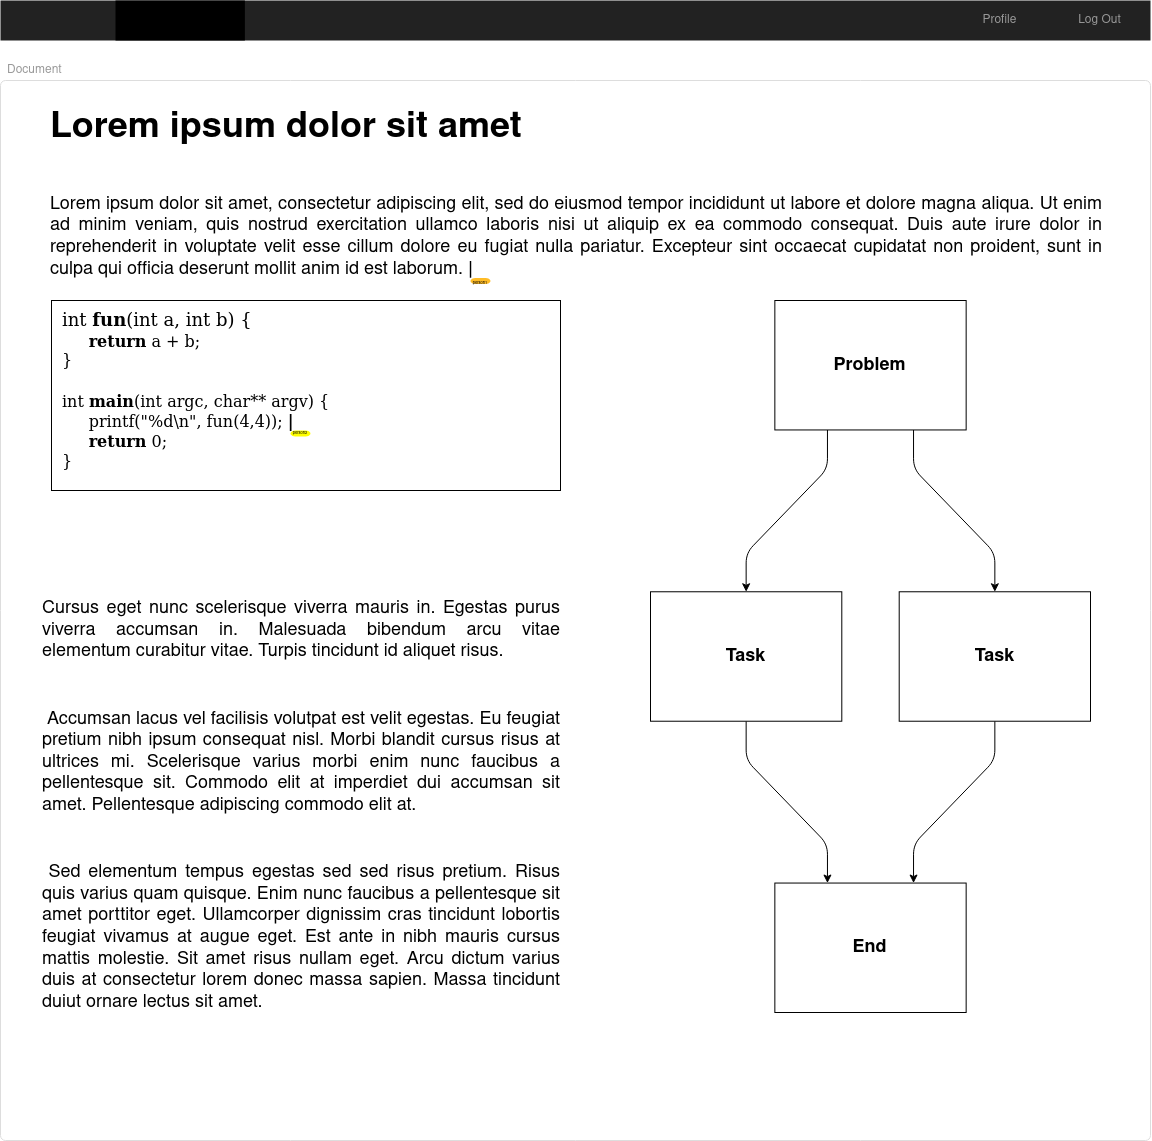
\includegraphics[width=0.88\textwidth]{images/Interface01.png}
    \end{figure}

\begin{itemize}
  \item \textbf{Planeación de proyectos de software}: al adjuntar código que esté
    relacionado con diagramas de flujo que representen el problema a resolver y las
    tareas (o proposiciones) asociadas para su compleción, o que denoten cómo estará
    organizado las funciones del programa (incluyendo con ello descripciones
    breves).
  \item \textbf{Editor de notas}: La organización en diagramas ayuda a que sirva como una
    aplicación para tomar notas cómoda y fácil de usar. Además, la incorporación de
    formatos para código, hace de esta una herramienta esencial para estudiantes
    de carreras que estén relacionadas con el desarrollo de software.
  \item \textbf{Depuración de código colaborativo}: La visualización colaborativa en
    diagramas del código escrito trae consigo una depuración rápida y básica para
    código no compilado que pretende plantear una idea inicial para dar solución
    a un problema.
\end{itemize}

\noindent
\textbf{\large Colaboración Concurrente}\\ %daniel

\textbf{Motivación:} El objetivo de la pizarra es fomentar la colaboración y el intercambio de ideas entre usuarios, para lo cual es fundamental que la pizarra permita la colaboración en tiempo real entre los usuarios.

\textbf{Objetivo:} Permitir que múltiples usuarios trabajen de manera simultanea en la pizarra.

\textbf{Compartir con enlace:} El usuario debe poder generar un enlace único para compartir la pizarra con otros usuarios. 

Solo los usuarios autenticados deben poder acceder a los enlaces. Si un usuario que no se encuentra autenticado o no posee una cuenta intenta acceder a un enlace, será dirigido al flujo de autenticación/registro y luego a la pizarra.
        
El usuario debe poder elegir el nivel de acceso que se concede a los usuarios con el enlace:
\begin{itemize}
    \item \textbf{Solo lectura:} Permite a los usuarios con el enlace ver la pizarra, pero no realizar cambios.
    \item \textbf{Edición:} Permite a los usuarios con el enlace ver y editar la pizarra.
\end{itemize}

El usuario debe poder revocar el acceso a la pizarra en cualquier momento.

\textbf{Visualización de la colaboración:} Los usuarios que se encuentren trabajando en una pizarra deben poder visualizar en tiempo real las modificaciones realizadas a la pizarra por otros usuarios.

\begin{itemize}
    \item \textbf{Indicador de presencia:} Los usuarios deben poder ver en la barra superior los avatares de los usuarios que están conectados a la pizarra.
    \item \textbf{Cursor en tiempo real:} Los usuarios deben poder ver los cursores de los demás usuarios en la pizarra para indicar dónde están trabajando.
\end{itemize}
\end{itemize}


\noindent
\textbf{\large Guardado Automático y Control de Versiones}\\ %kary

  \textbf{Motivación: }El guardado automático protege contra la pérdida de datos en caso de fallos del sistema, errores del usuario o eventos inesperados. El control de versiones permite a los usuarios trabajar juntos en la misma pizarra virtual de forma eficiente. Permite rastrear los cambios, deshacer errores y restaurar versiones anteriores. 

    \textbf{Objetivo:} Garantizar la seguridad de los datos, facilitar la colaboración y mejorar la productividad de los usuarios.
   \begin{itemize}
    \item  \textbf{Guardado Automático}\\
    El guardado automático protege contra la pérdida de datos en caso de fallos del sistema, errores del usuario o eventos inesperados. Para la frecuencia de los cambios está la posibilidad de que trabajo del usuario en la pizarra se guarde automáticamente con una frecuencia configurable.Opciones de frecuencia opcionales entre cada 5, 10 o 15 minutos.
    \item \textbf{Ubicación del archivo:} Los archivos guardados automáticamente se deben almacenar en un servidor seguro y accesible para el usuario. Opciones de ubicación recomendadas: nube privada(por ejemplo, Google Drive, Dropbox), servidor local o almacenamiento propio de la aplicación.
    \item \textbf{Notificaciones:}El usuario debe recibir una notificación cada vez que se guarde automáticamente su trabajo. La notificación indicará: fecha y hora del guardado, así como ubicación del archivo guardado.
    \item \textbf{Restauración de versiones:} El usuario debe poder restaurar una versión anterior de la pizarra en cualquier momento.
    \item \textbf{Historial de versiones:}El usuario debe poder acceder al historial de versiones y ver las diferencias entre cada versión. Opciones para acceder al historial de versiones: lista de versiones con fecha y hora, miniaturas visuales de cada versión y cursor a deslizar para comparar dos versiones.
           Opciones para restaurar una versión: seleccionar una versión de la lista de versiones, usar un atajo de teclado o botón de "Restaurar" en la barra de herramientas.
    \item \textbf{Revertir cambios:} El usuario debe poder deshacer los últimos cambios realizados en la pizarra.
           Opciones para deshacer cambios: Botón de "Deshacer" en la barra de herramientas o atajo de teclado.
    \end{itemize}
    
\noindent
\textbf{\large Pizarra expansible}\\ %mauro

\textbf{Motivación:} Al momento de trabajar en múltiples pizarras puede ser sencillo que se pierda información relevante durante los cambios de pizarra, si bien lo ideal sería que los temas pudieran agruparse en una pizarra en específico cada uno. Hay temas que requerirán más espacio debido a los múltiples elementos que pueden componer una tarea/tema con muchos componentes o pasos.

  \textbf{Objetivo:} La aplicación debe ofrecer más espacio en pizarra conforme los usuarios añadan elementos en pantalla (notas, inserciones de Latex, etc). Como característica adicional, la aplicación emitirá un aviso cuando una pizarra sea demasiado grande, para sugerir al usuario segmentar el tema en múltiples pizarras. El usuario puede solicitar espacio a demanda conforme elige qué sitios del proyecto conviene ampliar en una determinada dirección, de manera que las personas pueda elegir qué tanto van a requerir de la aplicación.


\noindent
\textbf{\large Registro de Usuarios} %ulises
\begin{itemize}
    \item \textbf{Motivación:} Para que los usuarios puedan guardar el progreso de su trabajo realizado y tener una experiencia mas personalizada y que se ajuste a cada uno de ellos, dichos usuarios deben poder crear una cuenta de usuario , en la cual sus datos quedaran guardados , sus pizarras en las que hayan hecho algún cambio se guardará en su cuenta y en un perfil personalizado para cada uno de estos usuarios.
    \item \textbf{Objetivo:} Permite que los desarrolladores puedan crear su cuenta con un correo electrónico y contraseña, de esta manera podrán acceder a su pizarra y a sus datos guardados. 
    \item \textbf{Función:} Los usuarios deben ser capaces de poder registrarse en la aplicación web de una manera cómoda , incluyendo su nombre de usuario, nombre de la persona , contraseña , además de incluir una forma de recuperar su cuenta , en caso de que el usuario pierda su contraseña, todo esto para brindar la mejor experiencia al usuario mientras usa la pizarra y todas sus funcionalidades.

    \item \textbf{Experiencia de usuario:}El registro por parte de los usuarios debe ser cómodo, intuitivo y fácil de usar, además de tener buena apariencia.
\end{itemize}


\noindent
\textbf{\large Soporte de \LaTeX y herramientas para graficar funciones}\\
    \textbf{Motivación: } En la colaboración entre personas de la academia puede resultar útil utilizar software especializado en expresar fórmulas matemáticas y agregar gráficas para hacer más claro un tema, en la actualidad si bien se utilizan múltiples tipos de pizarras para dar clase en línea y las fórmulas matemáticas pueden escribirse utilizando algún tipo de "pincel", esta no es la forma más eficaz de escribir pues en promedio una persona se tarda más tiempo escribiendo con esas herramientas que con un teclado común de computadora. Si nuestra aplicación busca resolver problemáticas colaborativas debe poder también hacer más eficaz el colaborar en términos de tiempo al momento de escribir, afortunadamente la aplicación incluir herramientas que sabemos que hacen la labor mucho más llevadera.\\
    \textbf{Objetivo:} La aplicación debe integrar herramientas que permitan usar fórmulas expresadas en
  \LaTeX, lo cual se complementa con el poder de hacer gráficas similares a las que se realizan en cursos básicos de cálculo; generalmente las gráficas tiene una función ilustrativa o ayudan mucho a comprender más cabalmente un concepto . La idea es que las personas que han tenido acercamientos a estas herramientas especializadas encuentren intuitivo agregar un segmento que compile el código en \LaTeX para mostrar en tiempo real cómo se interpretan las expresiones. De manera similar apoyarse en un graficador hace muy útil tener disponible información mutable y que se puede expresar a través de funciones.

%\noindent
%\textbf{Funcionalidades Avanzadas de Colaboración}\\
%  Facilita la interacción de usuarios a través de funcionalidades como
%  comentarios, menciones y notificaciones en tiempo real; promoviendo un
%  ambiente de trabajo colaborativo y eficiente.


\noindent
\textbf{\large Página de pizarras del usuario:}

\textbf{Motivación:} Aunque el acceso a las pizarras mediante enlace posibilita que se compartan las pizarras de una manera sencilla y flexible, es fácil que posteriormente se pierda el acceso al enlace o se olvide dónde se encuentra. Es necesario que el usuarios pueda acceder a sus pizarras y gestionarlas aunque ya no cuente con el enlace de acceso.

\textbf{Objectivo:} La página de pizarras tiene como objetivo centralizar la gestión y el acceso a los documentos del usuario, tanto aquellos creados por él mismo como aquellos que han sido compartidos con él por otros usuarios.

La página de pizarras muestra una lista de las pizarras del usuario. Para cada pizarra en la lista se muestra una tarjeta con el título, la fecha del último cambio realizado a la pizarra, y una miniatura del contenido de la pizarra. La tarjeta de la pizarra también incluye un botón para eliminarla. La función de eliminar la pizarra solo se muestra para las pizarras que haya creado el usuario. Las pizarras compartidas con el usuario solo pueden ser eliminadas por el usuario que las creó. 

También se incluye la opción de filtrar las pizarras para solo visualizar en la lista las pizarras creadas por el usuario, las compartidas con el usuario, o ambas.

  
\section{Objetivos futuros}

\section{Pantallas}
\end{document}